\chapter{Registri e Organizzazione della Memoria}

\section{Introduzione}

I registri sono celle di memoria ultrarapide integrate nel processore. L'8086 dispone di 14 registri a 16 bit, suddivisi in 4 categorie: registri generali, registri puntatore, registri indice e registri segmento. La conoscenza approfondita dei registri è fondamentale per scrivere codice Assembly efficiente.

\section{Registri General Purpose}

L'8086 ha 4 registri general purpose a 16 bit, ciascuno divisibile in due registri a 8 bit.

\subsection{Registro AX (Accumulatore)}

\begin{definizione}
\textbf{AX} è il registro \emph{accumulatore}, utilizzato per operazioni aritmetiche, I/O e moltiplicazioni/divisioni.
\end{definizione}

Il registro AX è un registro a 16 bit che può essere suddiviso in due sezioni: \textbf{AH} (byte alto - High) e \textbf{AL} (byte basso - Low). Questo design consente al programmatore di operare sia su dati a 16 bit usando AX nel suo complesso, sia su dati a 8 bit usando singolarmente AH per le cifre più significative e AL per quelle meno significative.

\begin{center}
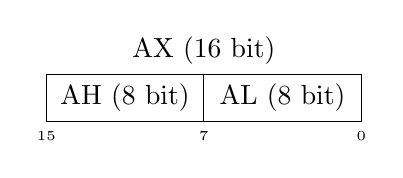
\begin{tikzpicture}
    \draw (0,0) rectangle (4,0.6);
    \draw (2,0) -- (2,0.6);
    \node at (1,0.3) {AH (8 bit)};
    \node at (3,0.3) {AL (8 bit)};
    \node[above] at (2,0.6) {AX (16 bit)};

    % Bit numbering
    \node[below, font=\tiny] at (0,0) {15};
    \node[below, font=\tiny] at (2,0) {7};
    \node[below, font=\tiny] at (4,0) {0};
\end{tikzpicture}
\end{center}

\textbf{Usi tipici}:

Il registro AX è fondamentale per molteplici operazioni. Innanzitutto, è il registro principale per le \emph{operazioni aritmetiche generiche}, poiché dispone di istruzioni ottimizzate per il calcolo. AX gioca anche un ruolo cruciale nelle \emph{istruzioni I/O}, dove AL viene utilizzato per leggere byte da una porta (\texttt{IN AL, port}) o scrivere byte su una porta (\texttt{OUT port, AL}). Nelle \emph{operazioni di moltiplicazione}, il registro AX contiene uno dei moltiplicandi e riceve il risultato: per moltiplicazioni a 8 bit il risultato risiede completamente in AX, mentre per moltiplicazioni a 16 bit il risultato si estende fino a DX:AX. Similmente, nelle \emph{operazioni di divisione}, AX funge da parte bassa del dividendo (per divisioni a 8 bit il dividendo è in AX; per divisioni a 16 bit è in DX:AX) e riceve il quoziente dopo la divisione.

\subsection{Registro BX (Base)}

Il registro BX è un registro a 16 bit suddiviso in \textbf{BH} (byte alto) e \textbf{BL} (byte basso), progettato specificamente come \emph{registro base per l'indirizzamento indiretto della memoria}.

\textbf{Usi tipici}:

BX rappresenta il registro preferito per l'\emph{indirizzamento di array}, permettendo di caricare dati dalla memoria con sintassi come \texttt{MOV AL, [BX]}. È frequentemente utilizzato come \emph{puntatore a strutture dati} complesse, consentendo di accedere ai vari campi della struttura combinando BX con offset. Oltre a questi ruoli specializzati, BX può essere impiegato per \emph{calcoli generici} come qualsiasi altro registro general purpose, offrendo così una versatilità che lo rende uno dei registri più utilizzati in Assembly.

\subsection{Registro CX (Contatore)}

Il registro CX è un registro a 16 bit suddiviso in \textbf{CH} (byte alto) e \textbf{CL} (byte basso), concepito come \emph{registro contatore per loop} e operazioni ripetitive.

\textbf{Usi tipici}:

CX è essenziale per le \emph{istruzioni di ciclo}, dove funge da contatore automaticamente decrementato dalle istruzioni \texttt{LOOP}, \texttt{LOOPE} e \texttt{LOOPNE}, permettendo al programma di ripetere blocchi di codice un numero specificato di volte. CX è anche il registro deputato al conteggio nelle \emph{operazioni su stringhe}, dove il prefisso \texttt{REP} utilizza CX per specificare quante volte ripetere un'istruzione come \texttt{MOVSB} o \texttt{STOSB}. Inoltre, CX è cruciale nelle \emph{operazioni di shift e rotate}, dove il registro CL (parte bassa di CX) specifica il numero di posizioni di cui spostare o ruotare un valore, consentendo shift e rotate dinamici.

\subsection{Registro DX (Dati)}

Il registro DX è un registro a 16 bit suddiviso in \textbf{DH} (byte alto) e \textbf{DL} (byte basso), progettato come \emph{registro dati per operazioni di I/O avanzate e calcoli estesi}.

\textbf{Usi tipici}:

DX è il registro specializzato per l'\emph{indirizzamento di porte I/O}, dove consente l'accesso a un grande numero di porte (fino a 65535) tramite istruzioni come \texttt{IN AL, DX} (per leggere da una porta il cui numero è in DX) e \texttt{OUT DX, AL} (per scrivere su una porta il cui numero è in DX). Nelle \emph{operazioni di moltiplicazione a 16 bit}, DX riceve la parte alta del risultato (mentre AX contiene la parte bassa), permettendo il calcolo di numeri molto grandi. Infine, nelle \emph{operazioni di divisione a 16 bit}, DX contiene la parte alta del dividendo insieme ad AX che contiene la parte bassa, formando così il registro a 32 bit DX:AX necessario per divisioni precise.

\subsection{Tabella riassuntiva}

\begin{table}[h]
\centering
\begin{tabular}{lllp{6cm}}
\toprule
\textbf{16 bit} & \textbf{8 bit H} & \textbf{8 bit L} & \textbf{Uso principale} \\
\midrule
AX & AH & AL & Accumulatore, I/O, moltiplicazioni \\
BX & BH & BL & Base per indirizzamento, puntatori \\
CX & CH & CL & Contatore loop, shift count \\
DX & DH & DL & Dati, porte I/O, divisioni \\
\bottomrule
\end{tabular}
\caption{Registri general purpose}
\end{table}

\section{Registri Puntatore e Indice}

Questi registri sono utilizzati per l'indirizzamento della memoria e non sono divisibili in byte.

\subsection{Stack Pointer (SP)}

\begin{definizione}
\textbf{SP} punta alla cima dello stack nel segmento SS. Lo stack cresce verso indirizzi decrescenti.
\end{definizione}

Il Stack Pointer è un registro specializzato per la gestione dello stack, una struttura dati LIFO (Last In, First Out) cruciale per la programmazione in Assembly. SP è utilizzato esclusivamente con le istruzioni \texttt{PUSH} e \texttt{POP}, che lo modificano automaticamente. Quando si esegue una \texttt{PUSH}, SP viene decrementato di 2 (per memorizzare una word di 16 bit), permettendo all'elemento di essere aggiunto in cima allo stack. Inversamente, una \texttt{POP} incrementa SP di 2 dopo aver recuperato l'elemento dalla cima dello stack. L'indirizzo fisico della cima dello stack è sempre calcolato combinando il registri segmento \texttt{SS} con l'offset \texttt{SP}, formando l'indirizzo \texttt{SS:SP}.

\subsection{Base Pointer (BP)}

Il Base Pointer è un \emph{puntatore base per accedere a parametri e variabili locali} all'interno dello stack frame di una procedura. BP è tipicamente utilizzato in combinazione con il segmento \texttt{SS} per accedere ai dati nello stack con indirizzamento del tipo \texttt{[BP+offset]}, dove l'offset specifica la posizione relativa rispetto alla cima dello stack frame. BP è \emph{fondamentale nelle chiamate a procedure}, dove viene salvato all'inizio di ogni procedura per stabilire un punto di riferimento fisso per l'accesso ai parametri e alle variabili locali, indipendentemente dalle modifiche apportate a SP durante l'esecuzione della procedura stessa.

\subsection{Source Index (SI)}

Il Source Index è un \emph{registro indice sorgente specializzato per operazioni su stringhe}. SI è principalmente utilizzato in combinazione con il segmento di dati \texttt{DS}, formando l'indirizzo \texttt{DS:SI}, per specificare la posizione dei dati sorgente. Il suo valore viene \emph{automaticamente incrementato o decrementato} quando viene utilizzato con istruzioni come \texttt{LODS} (Load String), \texttt{MOVS} (Move String) e \texttt{CMPS} (Compare String), permettendo di traversare facilmente una sequenza di byte o word in memoria senza dover gestire manualmente l'incremento dell'indice.

\subsection{Destination Index (DI)}

Il Destination Index è il \emph{registro indice destinazione utilizzato per operazioni su stringhe}. DI è solitamente utilizzato con il segmento extra \texttt{ES}, formando l'indirizzo \texttt{ES:DI}, per specificare dove i dati devono essere scritti o confrontati. Come SI, il valore di DI viene \emph{automaticamente modificato} (incrementato o decrementato) durante l'esecuzione di istruzioni come \texttt{STOS} (Store String), \texttt{MOVS} (Move String) e \texttt{SCAS} (Scan String), facilitando l'elaborazione sequenziale di stringhe.

\subsection{Instruction Pointer (IP)}

\begin{definizione}
\textbf{IP} contiene l'offset della prossima istruzione da eseguire nel segmento CS. Non è direttamente modificabile, ma cambia con istruzioni di salto e chiamate.
\end{definizione}

L'Instruction Pointer è un registro specializzato che non può essere direttamente letto o modificato dal programmatore, ma che governa completamente il flusso di esecuzione del programma. L'indirizzo fisico dell'istruzione corrente è sempre calcolato combinando il registro segmento \texttt{CS} con l'offset contenuto in \texttt{IP}, formando l'indirizzo \texttt{CS:IP}. Il valore di IP è modificato solamente da istruzioni di controllo del flusso: le istruzioni \texttt{JMP} (salti incondizionati) cambiano IP per saltare a una nuova posizione, le istruzioni \texttt{CALL} (chiamate a procedura) modificano IP durante la chiamata, \texttt{RET} (return da procedura) ripristina il valore precedente di IP, e gli interrupt (\texttt{INT} e \texttt{IRET}) modificano IP per gestire situazioni eccezionali. Dopo l'esecuzione di ogni istruzione ordinaria, IP viene \emph{automaticamente incrementato} per puntare alla prossima istruzione in sequenza.

\section{Registri Segmento}

I 4 registri segmento definiscono le basi dei segmenti di memoria.

\subsection{Code Segment (CS)}

Il \textbf{Code Segment} è il registro segmento che contiene le istruzioni del programma. L'indirizzo fisico di ogni istruzione è calcolato combinando CS con l'Instruction Pointer, formando \texttt{CS:IP}. CS è \emph{modificabile solo tramite istruzioni di salto far} (\texttt{JMP FAR}, \texttt{CALL FAR}) o istruzioni di return da procedure far (\texttt{RET FAR}), che cambiano sia CS che IP per consentire salti tra segmenti diversi.

\subsection{Data Segment (DS)}

Il \textbf{Data Segment} è il registro segmento predefinito che contiene le variabili globali del programma. DS è \emph{utilizzato implicitamente} da molte istruzioni di indirizzamento che referenziano registri come \texttt{[BX]}, \texttt{[SI]}, e \texttt{[DI]}, i quali per default calcolano il loro indirizzo fisico usando DS come segmento di base. A differenza di CS, DS può essere \emph{modificato dal programmatore} tramite l'istruzione \texttt{MOV DS, AX}, permettendo di accedere a diversi segmenti di dati durante l'esecuzione del programma.

\subsection{Stack Segment (SS)}

Lo \textbf{Stack Segment} è il registro segmento che definisce la base del segmento dello stack. La cima dello stack è sempre localizzata all'indirizzo \texttt{SS:SP}, calcolato combinando il valore di SS con il Stack Pointer. SS è \emph{usato implicitamente} dalle istruzioni \texttt{PUSH} e \texttt{POP}, nonché da istruzioni di indirizzamento che utilizzano il registro \texttt{[BP]}, che per default riferisce al segmento SS piuttosto che DS.

\subsection{Extra Segment (ES)}

L'Extra Segment è un \textbf{registro segmento aggiuntivo} comunemente utilizzato per operazioni su stringhe. ES è \emph{usato implicitamente} dal registro DI (Destination Index) nelle istruzioni di manipolazione di stringhe come \texttt{STOS}, \texttt{MOVS} e \texttt{SCAS}, permettendo di specificare il segmento destinazione. ES risulta particolarmente \emph{utile per copiare dati tra segmenti diversi}, poiché consente di leggere da un segmento (usando DS:SI) e scrivere in un altro (usando ES:DI) nella stessa operazione.

\begin{attenzione}
I registri segmento \textbf{non possono essere modificati direttamente}. Bisogna passare attraverso un registro general purpose:

\begin{lstlisting}
; CORRETTO
MOV AX, 1000h
MOV DS, AX

; ERRORE - non consentito
MOV DS, 1000h
\end{lstlisting}
\end{attenzione}

\section{Organizzazione della Memoria}

\subsection{Modello di memoria segmentata}

Lo spazio di indirizzamento dell'8086 (1 MB) è organizzato in segmenti sovrapposti:

\begin{center}
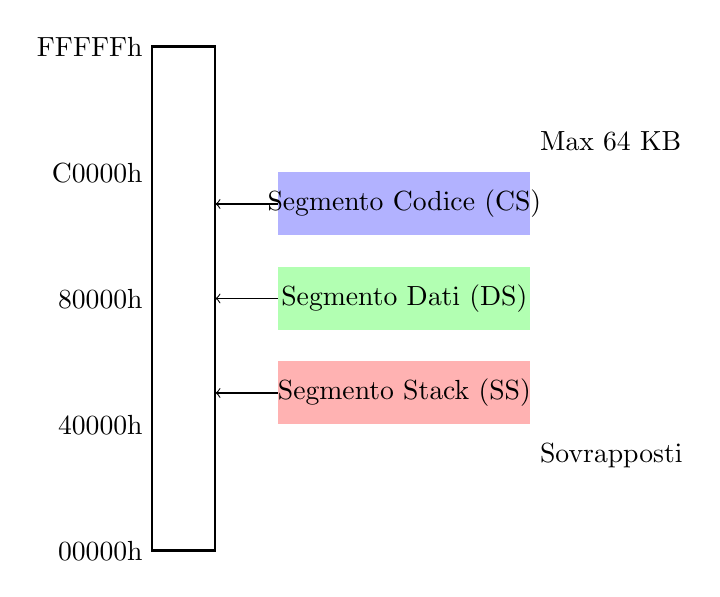
\begin{tikzpicture}[scale=0.8]
    % Memoria lineare
    \draw[thick] (0,0) rectangle (1,8);
    \node[left] at (0,8) {FFFFFh};
    \node[left] at (0,6) {C0000h};
    \node[left] at (0,4) {80000h};
    \node[left] at (0,2) {40000h};
    \node[left] at (0,0) {00000h};

    % Segmento codice
    \fill[blue!30] (2,5) rectangle (6,6);
    \node at (4,5.5) {Segmento Codice (CS)};

    % Segmento dati
    \fill[green!30] (2,3.5) rectangle (6,4.5);
    \node at (4,4) {Segmento Dati (DS)};

    % Segmento stack
    \fill[red!30] (2,2) rectangle (6,3);
    \node at (4,2.5) {Segmento Stack (SS)};

    % Frecce
    \draw[<-] (1,5.5) -- (2,5.5);
    \draw[<-] (1,4) -- (2,4);
    \draw[<-] (1,2.5) -- (2,2.5);

    \node[right] at (6,6.5) {Max 64 KB};
    \node[right] at (6,1.5) {Sovrapposti};
\end{tikzpicture}
\end{center}

\subsection{Layout tipico di un programma .COM}

\begin{center}
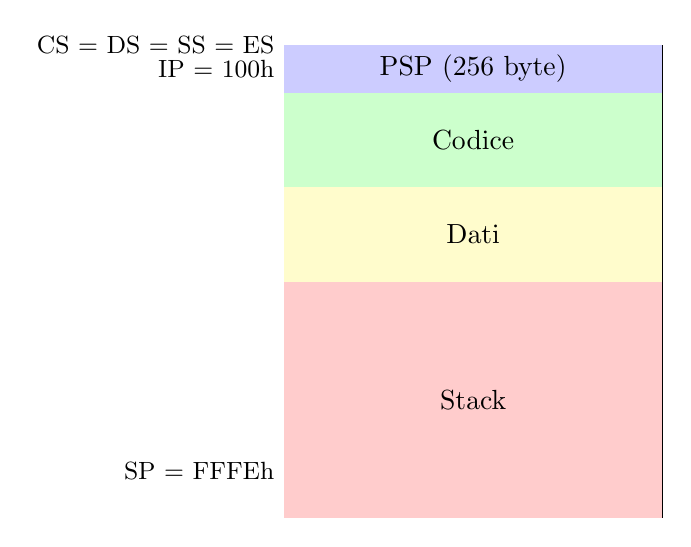
\begin{tikzpicture}[scale=1.2]
    \draw (0,0) rectangle (4,5);

    \fill[blue!20] (0,4.5) rectangle (4,5);
    \node at (2,4.75) {PSP (256 byte)};

    \fill[green!20] (0,3.5) rectangle (4,4.5);
    \node at (2,4) {Codice};

    \fill[yellow!20] (0,2.5) rectangle (4,3.5);
    \node at (2,3) {Dati};

    \fill[red!20] (0,0) rectangle (4,2.5);
    \node at (2,1.25) {Stack};

    \node[left, font=\small] at (0,5) {CS = DS = SS = ES};
    \node[left, font=\small] at (0,4.75) {IP = 100h};
    \node[left, font=\small] at (0,0.5) {SP = FFFEh};
\end{tikzpicture}
\end{center}

\begin{nota}
Nei programmi \textbf{.COM}, tutti i registri segmento puntano allo stesso indirizzo. L'intera immagine del programma (codice, dati, stack) risiede in un unico segmento di 64 KB. Il Program Segment Prefix (PSP) occupa i primi 256 byte.
\end{nota}

\subsection{Layout programma .EXE}

Nei file .EXE i segmenti hanno una struttura più complessa rispetto ai programmi .COM. Il \textbf{CS} (Code Segment) contiene le istruzioni del programma in una sezione dedicata. Il \textbf{DS} (Data Segment) è allocato separatamente per contenere le variabili globali, mantenendo una chiara separazione tra codice e dati. Lo \textbf{SS} (Stack Segment) è completamente separato da entrambi il segmento codice e il segmento dati, permettendo al programma di avere uno spazio stack ben definito e di dimensione appropriata. Infine, l'\textbf{ES} (Extra Segment) è tipicamente inizializzato allo stesso valore di DS all'avvio del programma, anche se può essere modificato durante l'esecuzione per operazioni su stringhe o per accedere a segmenti diversi.

\section{Convenzioni di utilizzo}

\begin{table}[h]
\centering
\small
\begin{tabular}{lp{9cm}}
\toprule
\textbf{Operazione} & \textbf{Registri tipici} \\
\midrule
Moltiplicazione 8 bit & AL 	imes operando $\rightarrow$ AX \\
Moltiplicazione 16 bit & AX 	imes operando $\rightarrow$ DX:AX \\
Divisione 8 bit & AX ÷ operando $\rightarrow$ AL (quoziente), AH (resto) \\
Divisione 16 bit & DX:AX ÷ operando $\rightarrow$ AX (quoziente), DX (resto) \\
Loop counter & CX (decrementato automaticamente) \\
String source & DS:SI \\
String destination & ES:DI \\
Procedure stack frame & SS:BP \\
I/O a 8 bit fisso & AL + numero porta immediato \\
I/O variabile & AL/AX + DX (numero porta) \\
\bottomrule
\end{tabular}
\caption{Convenzioni d'uso dei registri}
\end{table}

\section{Esempi pratici}

\begin{esempio}
Sommare due numeri a 16 bit:

\begin{lstlisting}
; Somma: 1234h + 5678h = 68ACh
MOV AX, 1234h     ; AX = 1234h
MOV BX, 5678h     ; BX = 5678h
ADD AX, BX        ; AX = 68ACh, BX immutato
\end{lstlisting}
\end{esempio}

\begin{esempio}
Accesso a byte alto e basso:

\begin{lstlisting}
MOV AX, 1234h     ; AX = 1234h
MOV BL, AL        ; BL = 34h (byte basso)
MOV BH, AH        ; BH = 12h (byte alto)
; Ora BX = 1234h
\end{lstlisting}
\end{esempio}

\begin{esempio}
Indirizzamento indiretto con BX:

\begin{lstlisting}
.DATA
array DB 10h, 20h, 30h, 40h

.CODE
MOV BX, OFFSET array   ; BX punta all'array
MOV AL, [BX]           ; AL = 10h (primo elemento)
INC BX                 ; BX punta al secondo elemento
MOV AL, [BX]           ; AL = 20h
\end{lstlisting}
\end{esempio}

\section{Riepilogo}

L'architettura dell'8086 dispone di 14 registri a 16 bit, ognuno specializzato in compiti specifici. I \emph{4 registri general purpose} (AX, BX, CX, DX) forniscono la flessibilità per operazioni di calcolo generiche e possono essere suddivisi in 8 coppie di byte (AH/AL, BH/BL, CH/CL, DH/DL) per operazioni su dati più piccoli. I \emph{registri puntatore e indice} hanno ruoli ben definiti: SP punta alla cima dello stack per le operazioni di push e pop, BP consente l'accesso ai parametri e alle variabili locali di una procedura, mentre SI e DI sono dedicati alle operazioni su stringhe. I \emph{4 registri segmento} (CS, DS, SS, ES) definiscono le basi dei diversi segmenti di memoria, permettendo l'accesso ai 1 MB di memoria totale tramite la combinazione di registro segmento e offset. Infine, IP contiene l'offset della prossima istruzione da eseguire e governa il flusso di esecuzione del programma. È importante notare che i \emph{programmi .COM utilizzano un unico segmento} dove codice, dati e stack coesistono, mentre i \emph{programmi .EXE hanno segmenti separati} per ciascuna di queste componenti, permettendo una migliore organizzazione e protezione dei dati.

\section{Esercizi}

\begin{esercizio}[2.1]
Dato \texttt{AX = 1234h}, scrivere le istruzioni per:
\begin{enumerate}[label=\alph*)]
    \item Azzerare solo AL mantenendo AH invariato
    \item Azzerare solo AH mantenendo AL invariato
    \item Scambiare AH e AL
\end{enumerate}
\end{esercizio}

\begin{esercizio}[2.2]
Spiegare la differenza tra \texttt{MOV AX, BX} e \texttt{MOV AX, [BX]}.
\end{esercizio}

\begin{esercizio}[2.3]
Perché non è possibile eseguire \texttt{MOV DS, 1000h}? Come si risolve?
\end{esercizio}

\begin{esercizio}[2.4]
Calcolare l'indirizzo fisico di \texttt{SS:SP = 2000h:FFFEh}. Se si esegue \texttt{PUSH AX}, qual è il nuovo valore di SP e l'indirizzo fisico corrispondente?
\end{esercizio}

\begin{esercizio}[2.5]
In un programma .COM, se tutti i segmenti valgono 1000h e IP = 0100h, qual è l'indirizzo fisico della prima istruzione?
\end{esercizio}
